\section{Theoretical guarantees}\label{sec:theory}

This section establishes three kinds of guarantees. The first is a worst-case limit that applies to \emph{every} online scheduler. The second is a set of worst-case and prediction-dependent guarantees for CARMA. The third is a fairness property of the carbon attribution induced by the pooled scheduling problem. Proofs are given in \ref{app:proofs}. Throughout, unit costs (Eq.~(\ref{eq:unitcost}), including any backstop resource introduced below) satisfy $0<L\le c_{os}(t)\le U$, and $\theta=U/L$ denotes the \emph{carbon-intensity ratio}. A positive floor $L$ holds as soon as the embodied emissions of servers, or a non-zero minimum grid intensity, are counted. An online algorithm is \emph{$\rho$-competitive} if its emissions never exceed $\rho$ times those of the clairvoyant oracle, for any arrival sequence and any intensity trajectory.

\subsection{A universal lower bound under demand uncertainty}\label{sec:lb}

Competitive analysis of carbon-aware scheduling has so far concentrated on uncertainty about future \emph{prices}, that is, future intensities, for a single workload. Examples are online search and one-way trading~\cite{elyaniv2001optimal}, the online pause-and-resume problem~\cite{lechowicz2023online} and spatiotemporal allocation with deadlines~\cite{lechowicz2025learning}. When several jobs share scarce low-carbon capacity, a second source of difficulty appears: uncertainty about \emph{future demand}. The next result shows that this uncertainty alone rules out good worst-case performance, however accurate the carbon forecasts are.

\begin{theorem}[Lower bound]\label{thm:lb}
Let $\theta\ge 1$. No online algorithm (deterministic or randomised, with integral or fractional decisions) can be better than $R^*(\theta)$-competitive, even if it knows all future carbon intensities exactly, where
\begin{equation}\label{eq:lb}
R^*(\theta)=\max_{1\le p\le\theta}\left\{1+\frac{(p-1)(\theta-p)}{p^2-p-1+\theta}\right\}\;\ge\;1+\frac{\sqrt\theta\,(\sqrt\theta-1)^2}{2\theta-\sqrt\theta-1}\;=\;\frac{\sqrt{\theta}}{2}+O(1).
\end{equation}
On the same instance, myopic receding-horizon scheduling (MPC) has ratio at least $(1+\theta)/2$.
\end{theorem}

The bound is attained on a two-hour instance, a quantitative version of Proposition~\ref{prop:myopic}. Any algorithm must decide how much flexible work to run now at moderate cost before it learns whether an urgent job will claim the cheap capacity later. For example, $R^*(100)=5.29$ and $R^*(1000)=16.1$, whereas the corresponding myopic ratios are 50.5 and 500.5. Theorem~\ref{thm:lb} also explains the empirical finding of Section~\ref{sec:res_main}: carbon forecasts cannot substitute for information about demand. It motivates the learning-augmented design of CARMA~\cite{lykouris2021competitive}, in which predictions of demand are used when they are good and cannot cause unbounded harm when they are bad.

\subsection{Robustness, consistency and smoothness of CARMA}\label{sec:guarantees}

We analyse CARMA under two assumptions.
\begin{itemize}
\item[(A1)] \emph{Backstop capacity.} In every hour, work may also run on a backstop resource of unlimited capacity at a unit cost in $[L,U]$. Examples are bursting to a public-cloud region or to reserve servers at a carbon-intensive site. All jobs, real and predicted, are \emph{window-feasible}, $w_j\le m_j(d_j-a_j)$. The penalties satisfy $\Pi>U$ for real jobs and $\Pi_g\ge U$ for ghost jobs. The implementation satisfies the latter, because $\Pi_g$ is 1.5 times the largest local unit cost, which exceeds every unit cost including transfer overheads.
\item[(A2)] \emph{Episode within the planning window.} The episode $\{0,\dots,T-1\}$ has length $T\le H$, as for a daily batch window, so every planning problem extends to the end of the episode.
\end{itemize}
To measure prediction quality at hour $t$, let $F_t$ be the set of jobs that actually arrive after $t$, and $\hat F_t$ the ghost jobs used by CARMA. Jobs are compared after splitting them into \emph{atoms} with proportional widths, which leaves every planning problem unchanged (\ref{app:proofs}). Let $d_t$ be the smallest total work of atoms that must be added to or removed from $\hat F_t$ to obtain $F_t$. Let $\varepsilon_t=\max_{\tau>t,o,s}|\hat c_{os}(\tau\,|\,t)-c_{os}(\tau)|$ be the carbon-cost forecast error, and $W_t$ the total work pending at $t$ plus the larger of the true and predicted future work.

\begin{theorem}[Guarantees for CARMA]\label{thm:carma}
Under (A1), for any arrival sequence and any predictions, CARMA completes every job by its deadline and is $\theta$-competitive (\emph{robustness}). If (A2) also holds, then
\begin{equation}\label{eq:smooth}
\mathrm{ALG}\;\le\;\min\Big\{\theta\cdot\mathrm{OPT},\;\;\mathrm{OPT}+\sum_{t=0}^{T-1}\big[(U-L)\,d_t+2\,\varepsilon_t\,W_t\big]\Big\}.
\end{equation}
In particular, with exact predictions ($d_t=\varepsilon_t=0$) CARMA is optimal (\emph{consistency}), and its excess emissions grow at most linearly in the prediction errors (\emph{smoothness}).
\end{theorem}

The three properties are the standard desiderata for algorithms with predictions~\cite{lykouris2021competitive,lechowicz2025learning}. Two features of the bound matter in practice. First, demand errors are paid at rate $U-L$, the spread of unit costs, not at the lateness penalty. This is because the backstop absorbs any misprediction, so a wrong prediction can make CARMA use dirtier capacity but can never make a real job late. Second, the bound does not depend on how the forecasts were produced, so it holds for the point and conformal cost views alike. Without demand predictions, myopic MPC has no consistency guarantee: by Theorem~\ref{thm:lb} it can be a factor of $(1+\theta)/2$ from optimal even with perfect carbon forecasts. Robustness $\theta$ is not optimal in view of the $\Theta(\sqrt\theta)$ lower bound. Closing this gap, for example by protecting deferral decisions with reservation prices in the spirit of~\cite{elyaniv2001optimal,lechowicz2025learning}, is left for future work. Assumption (A2) is needed only for the smoothness term, because horizon truncation couples decisions beyond the planning window. The experiments in Section~\ref{sec:res_robust} use weekly episodes with $H=24$ hours and test the degradation empirically. Fig.~\ref{fig:ratios} summarises the worst-case landscape.

\begin{figure}[t]
\centering
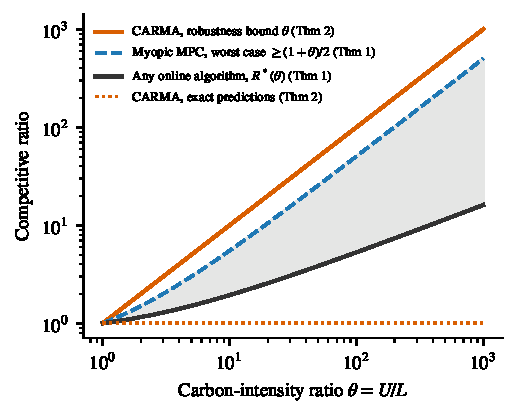
\includegraphics[width=0.62\textwidth]{../figures/fig7_ratios.pdf}
\caption{Worst-case landscape as a function of the carbon-intensity ratio $\theta$. No online algorithm can lie below $R^*(\theta)$ (Theorem~\ref{thm:lb}). Myopic MPC can be driven to $(1+\theta)/2$ even with perfect carbon forecasts. CARMA is never worse than $\theta$ (given a backstop) and is optimal when its predictions are exact (Theorem~\ref{thm:carma}).}
\label{fig:ratios}
\end{figure}

\subsection{Fair carbon attribution among sites}\label{sec:fair}

Pooling capacity reduces total emissions, but it redistributes them. Work from London is executed in South Scotland, and Scottish jobs may be displaced by it. The organisations that operate the sites (or the tenants that submit the jobs) therefore need an attribution of the pooled emissions that each of them can accept. We model this as a cooperative game. The players are the sites $\mathcal S$. A coalition $C\subseteq\mathcal S$ pools the capacity of its sites and serves the jobs submitted at them. Its stand-alone value $c(C)$ is the optimum of (\ref{eq:obj})--(\ref{eq:cap}) restricted to those jobs and sites. An attribution $\phi\in\mathbb{R}^{|\mathcal S|}$ is \emph{budget-balanced} if $\sum_o\phi_o=c(\mathcal S)$. It is in the \emph{core} if $\sum_{o\in C}\phi_o\le c(C)$ for every coalition $C$. A core attribution gives no group of sites a reason to leave the pool and schedule on its own.

Let $(\lambda,\nu,\mu)$ be optimal dual variables of the grand-coalition problem: $\lambda_j$ for the work constraint (\ref{eq:work}), $\nu_{jt}\le 0$ for the width constraint (\ref{eq:width}) and $\mu_{st}\le 0$ for the capacity constraint (\ref{eq:cap}). Define the \emph{dual carbon attribution}
\begin{equation}\label{eq:phi}
\phi_o=\sum_{j:\,o_j=o}\Big(\lambda_j w_j+\sum_t \nu_{jt}m_j\Big)+\sum_t\mu_{ot}K_o(t).
\end{equation}
Site $o$ is charged the carbon shadow price of the work it submits and is credited ($\mu\le 0$) with the shadow value of the capacity it contributes.

\begin{theorem}[Core-stable carbon attribution]\label{thm:core}
The attribution (\ref{eq:phi}) is budget-balanced and in the core of the pooling game. In particular, it is individually rational: no site is charged more than its stand-alone optimum $c(\{o\})$. It is obtained from the node potentials of the min-cost flow of Proposition~\ref{prop:flow}, at no extra computational cost.
\end{theorem}

The result follows from Owen's theorem on linear production games~\cite{owen1975core}. Games defined by network flows are known to be totally balanced~\cite{kalai1982totally}. Carbon reporting is done after the fact, so the hindsight game is the relevant object for accounting. The simpler \emph{location-based} attribution, in which each site is charged the emissions of its own jobs wherever they ran, carries no such guarantee. Section~\ref{sec:res_fair} shows that in practice it violates the core in every test week, whereas the dual attribution never does for the hindsight benchmark.
